% !TeX root = ../document.tex

\chapter{黎曼(内禀)曲率张量}
\begin{xiti}
	\item 放弃$\tensor{\nabla}{_a}$定义中的无挠性条件(e),
	\begin{enumerate}
		\item[(1)] 试证存在张量$\tensor{T}{^c_a_b}$(叫\textbf{挠率张量})使
		\begin{displaymath}
		\Nabla{a}\Nabla{b} f-\Nabla{b}\Nabla{a}f=-\tensor{T}{^c_a_b}\Nabla{c}f\qc \forall f\in \F.
		\end{displaymath}
		提示:令$\tensor{{\tilde{\nabla}}}{_a} $为无挠算符,模仿定理3-1-4证明中的推导。
		\item[(2)] 试证$\tensor{T}{^c_a_b}\tensor{u}{^a}\tensor{v}{^b}=u^a\Nabla{a}v^c-v^a\Nabla{a}u^c-{[u,v]}^c\quad \forall u^a,v^a\in\F(1,0) $。
	\end{enumerate}
	
	\begin{zm}
		\begin{enumerate}
			\item[(1)] 去掉无挠性条件仍有$\Nabla{a}\tensor{\omega}{_b}=\tensor{\tilde{\nabla}}{_a}\tensor{\omega}{_b}-\tensor{C}{^c_a_b}\tensor{\omega}{_c} $成立,于是令$\tensor{\omega}{_a}=\tensor{\left(\dd{f}\right)}{_a}=\Nabla{a}f=\tensor{\tilde{\nabla}}{_a}f $,得
			\begin{displaymath}
			\Nabla{a}\Nabla{b}f=\tNabla{a}\tNabla{b}f-\tensor{C}{^c_a_b}\Nabla{c}f
			\end{displaymath}
			交换指标$a,b$得
			\begin{displaymath}
			\Nabla{b}\Nabla{a}f=\tNabla{b}\tNabla{a}f-\tensor{C}{^c_b_a}\Nabla{c}f
			\end{displaymath}
			两式相减得
			\begin{displaymath}
			\Nabla{a}\Nabla{b}f-\Nabla{b}\Nabla{a}f=\left(\tensor{C}{^c_b_a}-\tensor{C}{^c_a_b} \right)\Nabla{c}f
			\end{displaymath}
			于是得挠率张量$\tensor{T}{^c_a_b}=\tensor{C}{^c_a_b}-\tensor{C}{^c_b_a} $。
			\item[(2)] 
			\begin{align*}
			[u,v](f)=&\; u(v(f))-v(u(f))\\
			=&\; u^b\Nabla{b}\left( v^a\Nabla{a}f \right)-v^a\Nabla{a}\left( u^b\Nabla{b}f \right)\\
			=&\; u^b\left(\Nabla{b}v^a\right)\Nabla{a}f+u^bv^a\Nabla{b}\Nabla{a}f-v^a\left(\Nabla{a}u^b \right)\Nabla{b}f-v^au^b\Nabla{a}\Nabla{b}f\\
			=&\tmu \left(u^b\Nabla{b}v^a-v^b\Nabla{b}u^a\right)\Nabla{a}f-u^b v^a \tensor{T}{^c_b_a}\Nabla{c}f\\
			=&\tmu \left( u^a\Nabla{a}v^c-v^a\Nabla{a}u^c-\tensor{T}{^c_a_b}u^a v^b \right)\Nabla{c}f
			\end{align*}
			故$\tensor{T}{^c_a_b}\tensor{u}{^a}\tensor{v}{^b}=u^a\Nabla{a}v^c-v^a\Nabla{a}u^c-{[u,v]}^c $。
		\end{enumerate}
	\end{zm}
	
	\item 设$v^a$为矢量场,$v^\mu $和${v^\prime}^\mu$为$v^a$在坐标系$\{x^\nu\}$和$\{{x^\prime}^\nu \} $的分量,$\tensor{A}{^\nu_\mu}\equiv \pdv*{v^\nu}{x^\mu} $,$\tensor{{A^\prime}}{^\nu_\mu}\equiv \pdv*{{v^\prime}^\nu}{{x^\prime}^\mu} $,试证$\tensor{A}{^\nu_\mu}$和$\tensor{{A^\prime}}{^\nu_\mu}$的关系一般而言不满足张量分量变换律。提示:利用$v^\nu $与${v^\prime}^\nu $之间的变换规律。
	
	\begin{zm}
		\begin{align*}
		\tensor{{A^\prime}}{^\nu_\mu}=&\;\pdv{{v^\prime}^\nu}{{x^\prime}^\mu}\\
		=&\;\pdv{x^\sigma}{{x^\prime}^\mu}\pdv{x^\sigma}(\pdv{{x^\prime}^\nu}{x^\rho}v^\rho)\\
		=&\;\pdv{x^\sigma}{{x^\prime}^\mu}\pdv{{x^\prime}^\nu}{x^\sigma}{x^\rho}v^\rho +\pdv{x^\sigma}{{x^\prime}^\mu}\pdv{{x^\prime}^\nu}{x^\rho}\pdv{v^\rho}{x^\sigma}\\
		=&\;\pdv{x^\sigma}{{x^\prime}^\mu}\pdv{{x^\prime}^\nu}{x^\sigma}{x^\rho}v^\rho +\pdv{x^\sigma}{{x^\prime}^\mu}\pdv{{x^\prime}^\nu}{x^\rho}\tensor{A}{^\rho_\sigma},
		\end{align*}
		可以看到相比于张量分量变换律多出了第一项。
	\end{zm}
	
	\item 试证定理3-1-7。
	
	\begin{zm}
		\begin{align*}
		\tensor{v}{^\nu_{;\mu}}=&\; \Nabla{a}\tensor{v}{^b}\tensor{\left(\dd{x^\nu}\right)}{_b}\tensor{\left(\pdv{x^\mu}\right)}{^a}\\
		=&\tmu \left( \Partial{a}v^b+\ChristoffelSymbol{b}{a}{c}v^c \right)\tensor{\left(\dd{x^\nu}\right)}{_b}\tensor{\left(\pdv{x^\mu}\right)}{^a}\\
		=&\; \tensor{v}{^\nu_{,\mu}}+\ChristoffelSymbol{\nu}{\mu}{\sigma}\tensor{v}{^\sigma},\\
		\tensor{\omega}{_\nu_{;\mu}}=&\; \Nabla{a}\tensor{\omega}{_b}\tensor{\left(\pdv{x^\mu}\right)}{^a}\tensor{\left(\pdv{x^\nu}\right)}{^b}\\
		=&\tmu \left(\Partial{a}\tensor{\omega}{_b}-\ChristoffelSymbol{c}{a}{b}\tensor{\omega}{_c} \right)\tensor{\left(\pdv{x^\mu}\right)}{^a}\tensor{\left(\pdv{x^\nu}\right)}{^b}\\
		=&\; \tensor{\omega}{_\nu_{,\mu}}-\ChristoffelSymbol{\sigma}{\mu}{\nu}\tensor{\omega}{_\sigma}.
		\end{align*}
	\end{zm}
	
	\item \hypertarget{3.4}{} 用下式定义$\ChristoffelSymbol{\sigma}{\mu}{\nu}$:$\displaystyle\tensor{\left(\pdv{x^\nu}\right)}{^b}\Nabla{b}\tensor{\left(\pdv{x^\mu}\right)}{^a}=\ChristoffelSymbol{\sigma}{\mu}{\nu}\tensor{\left(\pdv{x^\sigma}\right)}{^a} $,试证
	\begin{enumerate}
		\item[(a)] $\ChristoffelSymbol{\sigma}{\mu}{\nu}=\ChristoffelSymbol{\sigma}{\nu}{\mu}$(提示:利用$\Nabla{a}$的无挠性和坐标基矢间的对易性。);
		\item[(b)] $\tensor{v}{^\nu_{;\mu}}=\tensor{v}{^\nu_{,\mu}}+\ChristoffelSymbol{\nu}{\mu}{\beta}\tensor{v}{^\beta} $(注:这其实是克氏符的等价定义。)。
	\end{enumerate}
	
	\begin{zm}
		\begin{enumerate}
			\item[(a)] 交换指标$\mu,\nu$得
			\begin{displaymath}
			\tensor{\left(\pdv{x^\mu}\right)}{^b}\Nabla{b}\tensor{\left(\pdv{x^\nu}\right)}{^a}=\ChristoffelSymbol{\sigma}{\nu}{\mu}\tensor{\left(\pdv{x^\sigma}\right)}{^a}
			\end{displaymath}
			两式相减得:
			\begin{align*}
			\left(  \ChristoffelSymbol{\sigma}{\mu}{\nu}-\ChristoffelSymbol{\sigma}{\nu}{\mu} \right) \tensor{\left(\pdv{x^\sigma} \right)}{^a}= &\tmu  \tensor{\left(\pdv{x^\nu}\right)}{^b} \Nabla{b} \tensor{\left(\pdv{x^\mu}\right)}{^a}-\tensor{\left(\pdv{x^\mu}\right)}{^b} \Nabla{b} \tensor{\left(\pdv{x^\nu}\right)}{^a}\\
			=&\tmu \tensor{\left[\pdv{x^\nu},\pdv{x^\mu} \right]}{^a}\\
			=&\; 0,
			\end{align*}
			故$\ChristoffelSymbol{\sigma}{\mu}{\nu}=\ChristoffelSymbol{\sigma}{\nu}{\mu} $。
			\item[(b)] 由$$\tensor{\left(\pdv{x^\nu}\right)}{^b}\Nabla{b}\tensor{\left(\pdv{x^\mu}\right)}{^a}=\ChristoffelSymbol{\sigma}{\mu}{\nu}\tensor{\left(\pdv{x^\sigma}\right)}{^a}$$知$$\Nabla{b}\tensor{\left(\pdv{x^\mu}\right)}{^a}=\ChristoffelSymbol{\sigma}{\mu}{\nu}\tensor{\left(\dd{x^\nu}\right)}{_b} \tensor{\left(\pdv{x^\sigma}\right)}{^a}, $$于是
			\begin{align*}
			\Nabla{a} \tensor{v}{^b} 
			=&\; \Nabla{a} \left[ \tensor{v}{^\mu} \tensor{\left(\pdv{x^\mu}\right)}{^b} \right] \\
			=&\tmu \tensor{\left(\dd{v^\mu}\right)}{_a} \tensor{\left(\pdv{x^\mu}\right)}{^b} + \tensor{v}{^\mu} \Nabla{a} \tensor{\left(\pdv{x^\mu}\right)}{^b}\\
			=&\; \pdv{\tensor{v}{^\mu}}{x^\nu} \tensor{\left(\dd{x^\nu}\right)}{_a} \tensor{\left(\pdv{x^\mu}\right)}{^b} + \tensor{v}{^\mu} \ChristoffelSymbol{\sigma}{\mu}{\nu} \tensor{\left(\dd{x^\nu}\right)}{_a} \tensor{\left(\pdv{x^\sigma}\right)}{^b}\\
			=&\tmu \left(\pdv{\tensor{v}{^\mu}}{x^\nu} +  \ChristoffelSymbol{\mu}{\sigma}{\nu} \tensor{v}{^\sigma} \right) \tensor{\left(\dd{x^\nu}\right)}{_a} \tensor{\left(\pdv{x^\mu}\right)}{^b}
			\end{align*}
			于是$\Nabla{a}\tensor{v}{^b}$的分量$\tensor{v}{^\nu_{;\mu}}=\tensor{v}{^\nu_{,\mu}}+\ChristoffelSymbol{\nu}{\mu}{\sigma} \tensor{v}{^\sigma} $。
		\end{enumerate}
	\end{zm}
	
	\item 判断是非:
	\begin{enumerate}
		\item[(1)] \hypertarget{3.5.1}{}$\Nabla{a} \tensor{\left(\dd{x^\mu}\right)}{_b} =0 $;
		\item[(2)] $\tensor{v}{^\nu_{;\mu}} = \left(\Nabla{a} \tensor{v}{^b} \right) \tensor{\left(\pd{x^\mu} \right)}{^a} \tensor{\left(\dd{x^\nu}\right)}{_b} $;
		\item[(3)] $\tensor{v}{^\nu_{,\mu}} = \left(\Partial{a} \tensor{v}{^b} \right) \tensor{\left(\pd{x^\mu} \right)}{^a} \tensor{\left(\dd{x^\nu}\right)}{_b} $;
		\item[(4)] \hypertarget{3.5.4}{} $\tensor{v}{^\nu_{;\mu}}=\tensor{\left(\pd{x^\mu}\right)}{^a} \Nabla{a} \tensor{v}{^\nu} $;
		\item[(5)] $\tensor{v}{^\nu_{,\mu}}=\tensor{\left(\pd{x^\mu}\right)}{^a} \Nabla{a} \tensor{v}{^\nu} $。
	\end{enumerate}
	
	\begin{jie}
		\begin{enumerate}
			\item[(1)] 错。
			\begin{align*}
			\Nabla{a} \tensor{\left(\dd{x^\mu}\right)}{_b}&=\Partial{a} \tensor{\left(\dd{x^\mu}\right)}{_b} - \ChristoffelSymbol{c}{a}{b} \tensor{\left(\dd{x^\mu}\right)}{_c}\\
			&=0-\ChristoffelSymbol{\mu}{\nu}{\rho} \tensor{\left(\dd{x^\nu}\right)}{_a} \tensor{\left(\dd{x^\rho}\right)}{_b}
			\end{align*}
			不一定为零。
			\item[(2)] 根据定义知正确。
			\item[(3)] 根据定义知正确。
			\item[(4)] 不正确。(右边和$\Nabla{a}$的选择无关可直接判断)
			\begin{align*}
			\tensor{v}{^\nu_{;\mu}}&= \left(\Nabla{a} \tensor{v}{^b} \right) \tensor{\left(\pdv{x^\mu} \right)}{^a} \tensor{\left(\dd{x^\nu}\right)}{_b}\\
			&= \left[\Nabla{a} \tensor{v}{^\rho} \tensor{\left(\pdv{x^\rho}\right)}{^b} \right] \tensor{\left(\pdv{x^\mu} \right)}{^a} \tensor{\left(\dd{x^\nu}\right)}{_b}\\
			&=\left(\Nabla{a} \tensor{v}{^\rho} \right) \tensor{\left(\pdv{x^\mu} \right)}{^a} \tensor{\left(\dd{x^\nu}\right)}{_b} +\tensor{v}{^\rho} \left[ \Nabla{a} \tensor{\left( \pdv{x^\rho} \right)}{^b} \right] \tensor{\left(\pdv{x^\mu} \right)}{^a} \tensor{\left(\dd{x^\nu}\right)}{_b},
			\end{align*}
			多出来的后一项类似~\hyperlink{3.5.1}{(1)}~,一般不为零。
			\item[(5)] 正确,
			\begin{align*}
			\tensor{\left(\pdv{x^\mu}\right)}{^a} \Nabla{a} \tensor{v}{^\nu}&=\tensor{\left(\pdv{x^\mu}\right)}{^a} \tensor{\left(\dd{v^\nu}\right)}{_a} \\
			&=\tensor{\left(\pdv{x^\mu}\right)}{^a} \pdv{\tensor{v}{^\nu}}{x^\rho} \tensor{\left(\dd{x^\rho}\right)}{_a}\\
			&=\pdv{ \tensor{v}{^\nu}}{x^\mu}\\
			&=\tensor{v}{^\nu_{,\mu}}.
			\end{align*}
		\end{enumerate}
	\end{jie}
	
	\item 设$C(t) $是$\{x^\mu\}$的坐标域内的曲线,$x^\mu (t)$是$C(t)$在该系的参数表达式,$\tensor{v}{^a}$是$C(t)$上的矢量场,令$\mathrm{D}\tensor{v}{^\mu} / \dd{t} \equiv \tensor{\left(\dd{x^\mu}\right)}{_a} \tensor{\left(\pd{t}\right)}{^b} \Nabla{b} \tensor{v}{^a} $,试证
	\begin{displaymath}
	\mathrm{D} \tensor{v}{^\mu} / \dd{t} \equiv \dv*{\tensor{v}{^\mu}}{t} + \ChristoffelSymbol{\mu}{\nu}{\sigma} \tensor{v}{^\sigma} \dv*{x^\nu (t)}{t}.
	\end{displaymath}
	
	\begin{zm}
		由定理3-2-1,$\displaystyle \tensor{\left(\pdv{t}\right)}{^b} \Nabla{b} \tensor{v}{^a} = \tensor{\left(\pdv{x^\mu}\right)}{^a} \left( \dv{\tensor{v}{^\mu}}{t} + \ChristoffelSymbol{\mu}{\nu}{\sigma} \dv{x^\mu(t)}{t} \tensor{v}{^\sigma} \right) $,于是
		\begin{align*}
		\frac{\mathrm{D}\tensor{v}{^\mu}}{\dd{t}} &\equiv \tensor{\left(\dd{x^\mu}\right)}{_a} \tensor{\left(\pdv{t}\right)}{^b} \Nabla{b} \tensor{v}{^a}\\
		&=\tensor{\left(\dd{x^\mu}\right)}{_a} \tensor{\left(\pdv{x^\rho}\right)}{^a} \left( \dv{\tensor{v}{^\rho}}{t} + \ChristoffelSymbol{\rho}{\nu}{\sigma} \dv{x^\rho(t)}{t} \tensor{v}{^\sigma} \right)\\
		&= \dv{\tensor{v}{^\mu}}{t} + \ChristoffelSymbol{\mu}{\nu}{\sigma} \tensor{v}{^\sigma} \dv{x^\mu(t)}{t}  .
		\end{align*}
	\end{zm}
	
	\item \hypertarget{3.7}{}求出3维欧氏空间中球坐标系的全部非零$\ChristoffelSymbol{\sigma}{\mu}{\nu} $。
	
	\begin{jie}
		由\hyperlink{2.19a}{第二章19(a)}知,球坐标系下欧氏度规分量$\tensor{g}{_\mu_\nu}$排成的矩阵为:
		\begin{displaymath}
		\left[g\right]=\left(
		\begin{array}{ccc}
		1&0&0\\
		0&r^2&0\\
		0&0&r^2 \sin^2 \theta
		\end{array}
		 \right)
		\end{displaymath}
		取逆矩阵得$\tensor{g}{^\mu^\nu} $排成的矩阵为:
		\begin{displaymath}
		\left[g\right]^{-1}=\left(
		\begin{array}{ccc}
		1&0&0\\
		0&\frac{1}{r^2}&0\\
		0&0&\frac{1}{r^2 \sin^2 \theta}
		\end{array}
		\right)
		\end{displaymath}
		根据非对角元全为零,观察克氏符分量表达式
		\begin{displaymath}
		\ChristoffelSymbol{\sigma}{\mu}{\nu}=\christoffelSymbol{\sigma}{\mu}{\nu}{\rho}
		\end{displaymath}
		展开式中求和只有$\rho=\sigma$项才可能非零,于是
		\begin{displaymath}
		\ChristoffelSymbol{\sigma}{\mu}{\nu}=\christoffelSymbol{\sigma}{\mu}{\nu}{\sigma}
		\end{displaymath}
		($\sigma$是给定某个具体指标,不求和,也不需要指标平衡)若$\sigma\mu\nu$全不等,则括号内为零。
		于是那些可能非零的分量指标至少有两个相等:
		\begin{align*}
		\ChristoffelSymbol{r}{r}{r}=&\; \christoffelSymbol{r}{r}{r}{r}\\
		=&\; \frac{1}{2}\cdot 1 \cdot \left( 0+0-0 \right)\\\displaybreak[1]
		=&\; 0\\
		\ChristoffelSymbol{r}{r}{\theta}=&\; \christoffelSymbol{r}{r}{\theta}{r}\\
		=&\; \frac{1}{2} \cdot 1 \cdot \left( 0+0-0 \right)\\\displaybreak[1]
		=&\; 0\\
		\ChristoffelSymbol{r}{r}{\phi}=&\; \christoffelSymbol{r}{r}{\phi}{r}\\
		=&\; \frac{1}{2}\cdot 1\cdot \left( 0+0-0 \right)\\\displaybreak[1]
		=&\; 0\\
		\ChristoffelSymbol{r}{\theta}{\theta}=&\; \christoffelSymbol{r}{\theta}{\theta}{r}\\
		=&\; \frac{1}{2}\cdot 1\cdot \left( 0+0-2r \right)\\\displaybreak[1]
		=&\mspace{1mu}-\mspace{-4mu}r\\
		\ChristoffelSymbol{r}{\phi}{\phi}=&\; \christoffelSymbol{r}{\phi}{\phi}{r}\\
		=&\; \frac{1}{2}\cdot 1\cdot \left( 0+0-2r\sin^2\theta \right)\\
		=&\mspace{1mu} -\mspace{-4mu} r\sin^2\theta\\
		\ChristoffelSymbol{\theta}{r}{r}=&\; \christoffelSymbol{\theta}{r}{r}{\theta}\\
		=&\;0\\
		\ChristoffelSymbol{\theta}{r}{\theta}=&\; \christoffelSymbol{\theta}{r}{\theta}{\theta}\\
		=&\; \frac{1}{2}\cdot \frac{1}{r^2}\cdot \left( 0+2r-0 \right)\\
		=&\; \frac{1}{r}\\
		\ChristoffelSymbol{\theta}{\theta}{\theta}=&\; \christoffelSymbol{\theta}{\theta}{\theta}{\theta}\\
		=&\; 0\\
		\ChristoffelSymbol{\theta}{\theta}{\phi}=&\; \christoffelSymbol{\theta}{\theta}{\phi}{\theta}\\
		=&\; 0\\
		\ChristoffelSymbol{\theta}{\phi}{\phi}=&\; \christoffelSymbol{\theta}{\phi}{\phi}{\theta}\\
		=&\;\frac{1}{2}\cdot \frac{1}{r^2} \left( 0+0-2r^2 \cos\theta\sin \theta \right)\\
		=&\; -\cos\theta\sin\theta\\
		\ChristoffelSymbol{\phi}{r}{r}=&\; \christoffelSymbol{\phi}{r}{r}{\phi}\\\displaybreak[1]
		=&\; 0\\
		\ChristoffelSymbol{\phi}{r}{\phi}=&\; \christoffelSymbol{\phi}{r}{\phi}{\phi}\\
		=&\; \frac{1}{2}\cdot \frac{1}{r^2\sin^2\theta} \cdot \left( 0+2r\sin^2\theta-0 \right)\\\displaybreak[1]
		=&\; \frac{1}{r}\\
		\ChristoffelSymbol{\phi}{\theta}{\theta}=&\; \christoffelSymbol{\phi}{\theta}{\theta}{\phi}\\\displaybreak[1]
		=&\; 0\\
		\ChristoffelSymbol{\phi}{\theta}{\phi}=&\; \christoffelSymbol{\phi}{\theta}{\phi}{\phi}\\
		=&\; \frac{1}{2}\cdot \frac{1}{r^2\sin^2\theta}\cdot \left( 0+2r^2\cos\theta\sin\theta-0 \right)\\\displaybreak[1]
		=&\; \cot\theta\\
		\ChristoffelSymbol{\phi}{\phi}{\phi}=&\; \christoffelSymbol{\phi}{\phi}{\phi}{\phi}\\
		=&\; 0.
		\end{align*}
		故所有非零分量为$\displaystyle \ChristoffelSymbol{r}{\theta}{\theta}=-r $,$\displaystyle \ChristoffelSymbol{r}{\phi}{\phi}=-r \sin^2 \theta $,$\displaystyle \ChristoffelSymbol{\theta}{r}{\theta} = \ChristoffelSymbol{\theta}{\theta}{r} = \frac{1}{r} $,$\displaystyle \ChristoffelSymbol{\theta}{\phi}{\phi} = - \cos \theta \sin \theta $,$\displaystyle \ChristoffelSymbol{\phi}{r}{\phi} = \ChristoffelSymbol{\phi}{\phi}{r} = \frac{1}{r} $,$\displaystyle \ChristoffelSymbol{\phi}{\theta}{\phi} = \ChristoffelSymbol{\phi}{\phi}{\theta}=\cot\theta $。
	\end{jie}

	\item 设$I$是$\mathbb{R}$的一个区间,$C\colon I\rightarrow M $是$\left( M,\Nabla{a} \right)$中的曲线,试证$\forall s,t\in I $,平移映射$\psi\colon V_{C(s)}\rightarrow V_{C(t)} $(见图3-2)是同构映射。
	
	\begin{zm}
		对每个$v\in V_{C(s)}$,有唯一一个$C(t)$上的平移矢量场$\bar{v}(t)$满足$\bar{v}(s)=v$,$\psi(v)=v(t)$。首先易验证$\psi$为线性映射,下面论证$\ker\psi=\{0\}$。设$\psi(v)= \bar{v}(t)=0$,于是由正文(3-2-5)式:
		\begin{displaymath}
		\dvt{\tensor{\bar{v}}{^\mu}} + \ChristoffelSymbol{\mu}{\nu}{\sigma} \tensor{T}{^\nu}\tensor{\bar{v}}{^\sigma}=0 \qc \mu=1,\cdots ,n
		\end{displaymath}
		在$(s,t)$上此微分方程组的解被边界条件$\tensor{\bar{v}}{^\mu}(t)=0 $唯一确定,而$\tensor{\bar{v}}{^\mu}(t)\equiv0 $是解,于是知$v=\bar{v}(s)=0$,于是$\ker \psi=\{0\}$,又$\dim V_{C(s)}=\dim V_{C(t)}=n $,故线性映射$\psi $是同构映射。
	\end{zm}

	\item 试证定理3-3-2、3-3-3和3-3-5。
	
	\begin{zm}
		\begin{enumerate}
			\item[(1)] \hypertarget{3.9.1}{}定理3-3-2如下:
			\begin{yl}{{\heiti 定理}}
				设曲线$\gamma(t)$的切矢$\tensor{T}{^a} $满足$\tensor{T}{^b} \Nabla{b} \tensor{T}{^a} = \alpha \tensor{T}{^a} $[$\alpha$为$\gamma(t)$上的函数],则存在$t^\prime =t^\prime(t) $使得$\gamma^\prime (t^\prime )[=\gamma(t)] $为测地线。
			\end{yl}
		    证明如下:写出分量形式为
		    \begin{align*}
		    \tensor{T}{^b} \Nabla{b} \tensor{T}{^a} =& \tmu \left( \dv{\tensor{T}{^\mu}}{t} + \ChristoffelSymbol{\mu}{\nu}{\sigma} \tensor{T}{^\nu} \tensor{T}{^\sigma} \right) \tensor{\left( \pdv{x^\mu} \right)}{^a}\\
		    =&\tmu \left( \dv[2]{x^\mu}{t} + \ChristoffelSymbol{\mu}{\nu}{\sigma} \dv{x^\nu}{t} \dv{x^\sigma}{t} \right) \tensor{\left( \pdv{x^\mu} \right)}{^a}\\
		    \alpha \tensor{T}{^a}=&\; \tensor{T}{^\mu} \tensor{\left( \pdv{x^\mu} \right)}{^a}\\
		    =&\; \alpha \dv{x^\mu}{t} \tensor{\left( \pdv{x^\mu} \right)}{^a}\\
		    \implies \alpha \dv{x^\mu}{t}=&\; \dv[2]{x^\mu}{t} + \ChristoffelSymbol{\mu}{\nu}{\sigma} \dv{x^\nu}{t} \dv{x^\sigma}{t}
		    \end{align*}
		    设有重参数化$t^\prime=t^\prime (t) $使得$\gamma^\prime(t^\prime) $为测地线,则
		    \begin{align*}
		    \displaybreak[1]
		    \dv[2]{x^\mu}{{t^\prime}} + \ChristoffelSymbol{\mu}{\nu}{\sigma} \dv{x^\nu}{t^\prime} \dv{x^\sigma}{t^\prime}=&\; \dv{{t^\prime}} \left( \dv{t}{t^\prime } \dv{x^\mu}{t} \right) + \ChristoffelSymbol{\mu}{\nu}{\sigma} \left( \dv{t}{t^\prime} \dv{x^\nu}{t} \right) \left( \dv{t}{t^\prime} \dv{x^\sigma}{t} \right) \\\displaybreak[1]
		    =& \; \dv[2]{t}{{t^\prime}} \dv{x^\mu}{t} + \left( \dv{t}{t^\prime} \right)^2 \dv[2]{x^\mu}{t} + \left( \dv{t}{t^\prime} \right)^2  \ChristoffelSymbol{\mu}{\nu}{\sigma} \dv{x^\nu}{t} \dv{x^\sigma}{t}\\\displaybreak[1]
		    =&\; \left[ \dv[2]{t}{{t^\prime}} + \alpha \left( \dv{t}{t^\prime} \right)^2 \right] \dv{x^\mu}{t} \\
		    =&\; 0
		    \end{align*}
		    只要解微分方程$ \displaystyle \dv[2]{t}{{t^\prime}} + \alpha \left( \dv{t}{t^\prime} \right)^2=0 $,令$ \eta(t) =\dv{t^\prime}{t} $,则
		    \begin{displaymath}
		    \frac{1}{\eta} \dv{\eta}{t}+\alpha(t) \eta^2=0
		    \end{displaymath}
		    解得\[\eta(t)= \sqrt{2 \int \alpha(t) \dd{t}+C_1 }\]积分即得重参数化\[t^\prime(t)= \int\sqrt{2\int\alpha(t)\dd{t}+C_1}\dd{t}+C_2 \]其中积分均代表某个原函数,而不是不定积分。
		    \item[(2)] 定理3-3-3如下:
		    \begin{yl}{{\heiti 定理}}
		    	\hypertarget{th3-3-3}{}若$t$是某测地线的仿射参数,则该曲线的任一参数$t^\prime $是仿射参数的充要条件为$t^\prime =a t+b $(其中$a,b$为常数且$a\neq 0 $)。
		    \end{yl}
	        证明如下:完全类似~\hyperlink{3.9.1}{(1)}~,只是$\alpha(t)=0 $,于是微分方程为
	        $$ \dv[2]{t}{{t^\prime}}=0, $$解得$t^\prime=a t+b $。
	        \item[(3)] 定理3-3-5如下:
	        \begin{yl}{{\heiti 定理}}
	        	测地线的弧长参数必为仿射参数。
	        \end{yl}
            证明如下:设$t$为仿射参数,则$\displaystyle \tensor{T}{^b} \Nabla{b} \tensor{T}{^a} =0 $,于是
            \begin{align*}
            \tensor{T}{^a} \Nabla{a} \left( \tensor{g}{_b_c} \tensor{T}{^b} \tensor{T}{^c} \right) &=\tensor{g}{_b_c} \tensor{T}{^a} \tensor{T}{^b} \Nabla{a} \tensor{T}{^c} + \tensor{g}{_b_c} \tensor{T}{^a} \tensor{T}{^c} \Nabla{a} \tensor{T}{^b} \\
            &=0,
            \end{align*}
            于是$\tensor{g}{_a_b} \tensor{T}{^a} \tensor{T}{^b} $沿线为常数$T$,弧长按定义与$t$的关系为$ \dd{l} = \sqrt{ \abs{ \tensor{g}{_a_b} \tensor{T}{^a} \tensor{T}{^b} }} \dd{t}=T\dd{t} $,由定理~\hyperlink{th3-3-3}{3-3-3}~知$l$为仿射参数。
		\end{enumerate}
	\end{zm}
	
	\item \begin{enumerate}
		\item[(a)] \hypertarget{2.10}{}写出球面度规$\dd{s}^2=R^2 \left( \dd{\theta}^2 +\sin^2 \theta \dd{\phi}^2 \right) $($R$为常数)的测地线方程;
		\item[(b)] 验证任一大圆弧(配以适当参数)满足测地线方程。提示:选球面坐标系$\{\theta,\phi \} $使所给大圆弧为赤道的一部分,并以$\phi$为仿射参数。
	\end{enumerate}
    
    \begin{jie}
    	\begin{enumerate}
    		\item[(a)] 首先求克氏符,度规分量$\tensor{g}{_\mu_\nu}$排成的矩阵为
    		\begin{displaymath}
    		\left[g\right]=\left(
    		\begin{array}{cc}
    		R^2&0\\
    		0&R^2 \sin^2\theta 
    		\end{array}
    		\right)
    		\end{displaymath}
    		逆矩阵
    		\begin{displaymath}
    		\left[g\right]^{-1}=\left(
    		\begin{array}{cc}
    		\dfrac{1}{R^2}&0\\
    		0&\dfrac{1}{R^2 \sin^2\theta} 
    		\end{array}
    		\right)
    		\end{displaymath}
    		完全类似第~\hyperlink{3.7}{7}~题,根据非对角元全为零,观察克氏符分量表达式
    		\begin{displaymath}
    		\ChristoffelSymbol{\sigma}{\mu}{\nu}=\christoffelSymbol{\sigma}{\mu}{\nu}{\rho}
    		\end{displaymath}
    		展开式中求和只有$\rho=\sigma$项才可能非零,于是
    		\begin{displaymath}
    		\ChristoffelSymbol{\sigma}{\mu}{\nu}=\christoffelSymbol{\sigma}{\mu}{\nu}{\sigma}
    		\end{displaymath}
    		($\sigma$是给定某个具体指标,不求和,也不需要指标平衡)
    		\begin{align*}
    		\ChristoffelSymbol{\theta}{\theta}{\theta}&= \christoffelSymbol{\theta}{\theta}{\theta}{\theta}\\
    		&=0\\
    		\ChristoffelSymbol{\theta}{\theta}{\phi}&= \christoffelSymbol{\theta}{\theta}{\phi}{\theta}\\
    		&=0\\
    		\ChristoffelSymbol{\theta}{\phi}{\phi}&= \christoffelSymbol{\theta}{\phi}{\phi}{\theta}\\
    		&=\frac{1}{2}\cdot \frac{1}{R^2} \cdot \left( 0+0-2 R^2 \sin \theta \cos \theta \right)\\
    		&=-\sin\theta\cos\theta\\
    		\ChristoffelSymbol{\phi}{\theta}{\theta}&= \christoffelSymbol{\phi}{\theta}{\theta}{\phi}\\
    		&=0\\
    		\ChristoffelSymbol{\phi}{\theta}{\phi}&= \christoffelSymbol{\phi}{\theta}{\phi}{\phi}\\
    		&=\frac{1}{2}\cdot \frac{1}{R^2 \sin^2\theta} \cdot \left( 0+2R^2\sin\theta\cos\theta-0 \right)\\
    		&=\cot\theta\\
    		\ChristoffelSymbol{\phi}{\phi}{\phi}&= \christoffelSymbol{\phi}{\phi}{\phi}{\phi}\\
    		&=0
    		\end{align*}
    		代入测地线方程$\displaystyle \dv[2]{x^\mu}{t} + \ChristoffelSymbol{\mu}{\nu}{\sigma} \dv{x^\nu}{t} \dv{x^\sigma}{t}=0 $,
    		\begin{gather*}
    		\dv[2]{\theta}{t}-\sin \theta \cos \theta \left( \dv{\phi}{t} \right)^2 =0\\
    		\dv[2]{\phi}{t}+\cot\theta \dv{\theta}{t} \dv{\phi}{t} =0
    		\end{gather*}
    		\item[(b)] 由于测地线方程具有坐标系无关的形式$\tensor{T}{^b} \Nabla{b} \tensor{T}{^a}=0 $,可选择球坐标系使得大圆弧落在赤道$\theta=\dfrac{\pi}{2} $上,于是$\cos \theta=0 $,满足测地线方程。
    	\end{enumerate}
    \end{jie}
	
	\item 试证定理3-4-2.
	
	\begin{zm}
		在某坐标系下展开即得
		\begin{align*}
		{\left. \left[ \left( \Nabla{a} \Nabla{b} - \Nabla{b} \Nabla{a} \right) \tensor{\omega}{_c} \right] \right|}_p&={\left. \left[ \left( \Nabla{a} \Nabla{b} - \Nabla{b} \Nabla{a} \right) \tensor{\omega}{_\mu} \tensor{\left(\dd{x^\mu}\right)}{_c} \right] \right|}_p\\
		&={\left. \left[\tensor{\omega}{_\mu} \left( \Nabla{a} \Nabla{b} - \Nabla{b} \Nabla{a} \right)  \tensor{\left(\dd{x^\mu}\right)}{_c} \right] \right|}_p\quad(\text{由定理3-4-1})\\
		&=\tensor{\omega}{_\mu}|_p {\left. \left[ \left( \Nabla{a} \Nabla{b} - \Nabla{b} \Nabla{a} \right)  \tensor{\left(\dd{x^\mu}\right)}{_c} \right] \right|}_p
		\end{align*}
		可见只与$\omega$在$p$点的值有关,证毕。
	\end{zm}
	
	\item 试证式(3-4-10)。
	
	\begin{zm}
		首先,$\tensor{R}{_{[abc]}_d}= \tensor{g}{_d_e} \tensor{R}{_{[abc]}^e} =0 $,而
		\begin{align*}
		\tensor{R}{_{[abc]}_d}&=\frac{1}{6} \left( \tensor{R}{_a_b_c_d}+ \tensor{R}{_c_a_b_d}+ \tensor{R}{_b_c_a_d}- \tensor{R}{_a_c_b_d}- \tensor{R}{_b_a_c_d}- \tensor{R}{_c_b_a_d} \right)\\
		&=\frac{1}{3} \left( \tensor{R}{_a_b_c_d}+ \tensor{R}{_c_a_b_d}+ \tensor{R}{_b_c_a_d} \right)
		\end{align*}
		于是
		\begin{align*}
		&\;\tensor{R}{_{[abc]}_d} + \tensor{R}{_{[dab]c}} + \tensor{R}{_{[cda]b}} + \tensor{R}{_{[bcd]a}}\\
		=&\; \frac{1}{3} \left( \tensor{R}{_a_b_c_d}+ \tensor{R}{_c_a_b_d}+ \tensor{R}{_b_c_a_d} \right)+\frac{1}{3} \left( \tensor{R}{_d_a_b_c}+ \tensor{R}{_b_d_a_c}+ \tensor{R}{_a_b_d_c} \right)\\
		&+\frac{1}{3} \left( \tensor{R}{_c_d_a_b}+ \tensor{R}{_a_c_d_b}+ \tensor{R}{_d_a_c_b} \right)+\frac{1}{3} \left( \tensor{R}{_b_c_d_a}+ \tensor{R}{_d_b_c_a}+ \tensor{R}{_c_d_b_a} \right) \\
		=&\; \frac{1}{3} \left( \tensor{R}{_a_b_c_d}- \tensor{R}{_a_c_b_d}+ \tensor{R}{_b_c_a_d}- \tensor{R}{_d_a_c_b}+ \tensor{R}{_b_d_a_c}- \tensor{R}{_a_b_c_d}\right.\\
		&\left.+\tensor{R}{_c_d_a_b}- \tensor{R}{_a_c_b_d}+ \tensor{R}{_d_a_c_b}- \tensor{R}{_b_c_a_d}+ \tensor{R}{_b_d_a_c}- \tensor{R}{_c_d_a_b} \right)\\
		=&\; \frac{2}{3} \left( \tensor{R}{_b_d_a_c}- \tensor{R}{_a_c_b_d} \right)\\
		=&\;0
		\end{align*}
		于是$\tensor{R}{_b_d_a_c}- \tensor{R}{_a_c_b_d}=0$。
	\end{zm}
	
	\item \hypertarget{2.13}{}求出球面度规(见题~\hyperlink{2.10}{10}~)的黎曼张量在坐标系$(\theta,\phi)$的全部分量。
	
	\begin{jie}
		由~\hyperlink{2.10}{10}~得,克氏符的全部非零分量为$ \ChristoffelSymbol{\theta}{\phi}{\phi}=-\sin \theta \cos \theta,\ChristoffelSymbol{\phi}{\phi}{\theta}=\ChristoffelSymbol{\phi}{\theta}{\phi}=\cot \theta $,由$\tensor{R}{_{\mu\nu\sigma}^\rho}= \tensor{\Gamma}{^\rho_\mu_\sigma_{,\nu}}- \tensor{\Gamma}{^\rho_\nu_\sigma_{,\mu}}+ \ChristoffelSymbol{\lambda}{\sigma}{\mu} \ChristoffelSymbol{\rho}{\nu}{\lambda}- \ChristoffelSymbol{\lambda}{\sigma}{\nu} \ChristoffelSymbol{\rho}{\mu}{\lambda} $得,非零分量或者满足$\rho=\theta$且$\mu\nu\sigma $中有两个为$ \phi$,或者满足$\rho=\phi $且$\mu \nu \sigma $中至少有一个为$\theta$,且前两个指标反称,前两个指标相同的分量为零,并且前三个指标只需考虑偶排列,奇排列只需对调前两个指标。
		\begin{align*}
		\tensor{R}{_\theta_\phi_\phi^\theta}=&\; \riemannR{\theta}{\phi}{\phi}{\theta}{\theta}+ \ChristoffelSymbol{\phi}{\phi}{\theta} \ChristoffelSymbol{\theta}{\phi}{\phi}- \ChristoffelSymbol{\phi}{\phi}{\phi} \ChristoffelSymbol{\theta}{\theta}{\phi}\\
		=&\; 0+\left(\cos^2\theta-\sin^2\theta\right) +0-0-\cos^2\theta-0\\\displaybreak[1]
		=&\mspace{1mu}-\mspace{-1mu}\sin^2\theta\\
		\tensor{R}{_\theta_\phi_\phi^\phi}=&\; \riemannR{\theta}{\phi}{\phi}{\phi}{\theta}+ \ChristoffelSymbol{\phi}{\phi}{\theta} \ChristoffelSymbol{\phi}{\phi}{\phi}- \ChristoffelSymbol{\phi}{\phi}{\phi} \ChristoffelSymbol{\phi}{\theta}{\phi}\\\displaybreak[1]
		=&\; 0\\
		\tensor{R}{_\phi_\theta_\theta^\phi}=&\; \riemannR{\phi}{\theta}{\theta}{\phi}{\theta} + \ChristoffelSymbol{\phi}{\theta}{\phi} \ChristoffelSymbol{\phi}{\theta}{\phi} - \ChristoffelSymbol{\phi}{\theta}{\theta} \ChristoffelSymbol{\phi}{\phi}{\phi}\\
		=&\mspace{1mu}-\mspace{-4mu} \frac{1}{\sin^2\theta} - 0 + 0 - 0 + \cot^2 \theta - 0\\ \displaybreak[1]
		=&\mspace{1mu}-\mspace{-4mu}1
		\end{align*}
		于是非零分量仅有$\tensor{R}{_\theta_\phi_\phi^\theta}=-\tensor{R}{_\phi_\theta_\phi^\theta}=-\sin\theta, \tensor{R}{_\phi_\theta_\theta^\phi} = - \tensor{R}{_\theta_\phi_\theta^\phi}=-1 $。
		
		与愚蠢的人类相比,麦酱可以更快地计算(并且不会抄错分量\wl{12})。将以下函数定义写入一个Mathematica程序包文件(.m)或者放在笔记本文件的开头:
		\begin{lstlisting}[language=Mathematica]
'\mma christoffelsymbol'['\mmacs g\_','\mmacs x\_','\mmacs i\_','\mmacs j\_','\mmacs k\_']:=
   1/2
     '\mma Plus'@@
       ((Inverse['\mmacs g'][['\mmacs i','\mmacs \#']](D['\mmacs g'[['\mmacs \#','\mmacs j']],'\mmacs x'[['\mmacs k']]]+D['\mmacs g'[['\mmacs k','\mmacs \#']],'\mmacs x'[['\mmacs j']]]-
              D['\mmacs g'[['\mmacs j','\mmacs k']],'\mmacs x'[['\mmacs \#']]]))&)/@'\mma Range'[Length['\mmacs x']];
'\mma ChristoffelSymbol'['\mmacs g\_','\mmacs x\_']:=
   Table[christoffelsymbol['\mmacs g','\mmacs x','\mmab i','\mmab j','\mmab k'],{'\mmab i',1,Length['\mmacs x']},
      {'\mmab j',1,Length['\mmacs x']},{'\mmab k',1,Length['\mmacs x']}];
'mma riemanntensor'['\mmacs g\_','\mmacs x\_','\mmacs i\_','\mmacs j\_','\mmacs k\_','\mmacs l\_']:=
   D[christoffelsymbol['\mmacs g','\mmacs x','\mmacs l','\mmacs i','\mmacs k'],'\mmacs x'[['\mmacs j']]]-
    D[christoffelsymbol['\mmacs g','\mmacs x','\mmacs l','\mmacs j','\mmacs k'],'\mmacs x'[['\mmacs i']]]+
    '\mma Plus'@@
      ((christoffelsymbol['\mmacs g','\mmacs x','\mmacs \#','\mmacs k','\mmacs i'] christoffelsymbol['\mmacs g','\mmacs x','\mmacs l','\mmacs j','\mmacs \#']-
          christoffelsymbol['\mmacs g','\mmacs x','\mmacs \#','\mmacs k','\mmacs j']
           christoffelsymbol['\mmacs g','\mmacs x','\mmacs l','\mmacs i','\mmacs \#'])&)/@Range[Length['\mmacs x']];
RiemannTensor['\mmacs g\_','\mmacs x\_']:=Table[riemanntensor['\mmacs g','\mmacs x','\mmab i','\mmab j','\mmab k','\mmab l'],
    {'\mmab i',1,Length['\mmacs x']},{'\mmab j',1,Length['\mmacs x']},{'\mmab k',1,Length['\mmacs x']},{'\mmab l',1,Length['\mmacs x']}];
		\end{lstlisting}
		运行如图~\ref{f3.1}。
		\begin{figure}[htb]
			\centering
			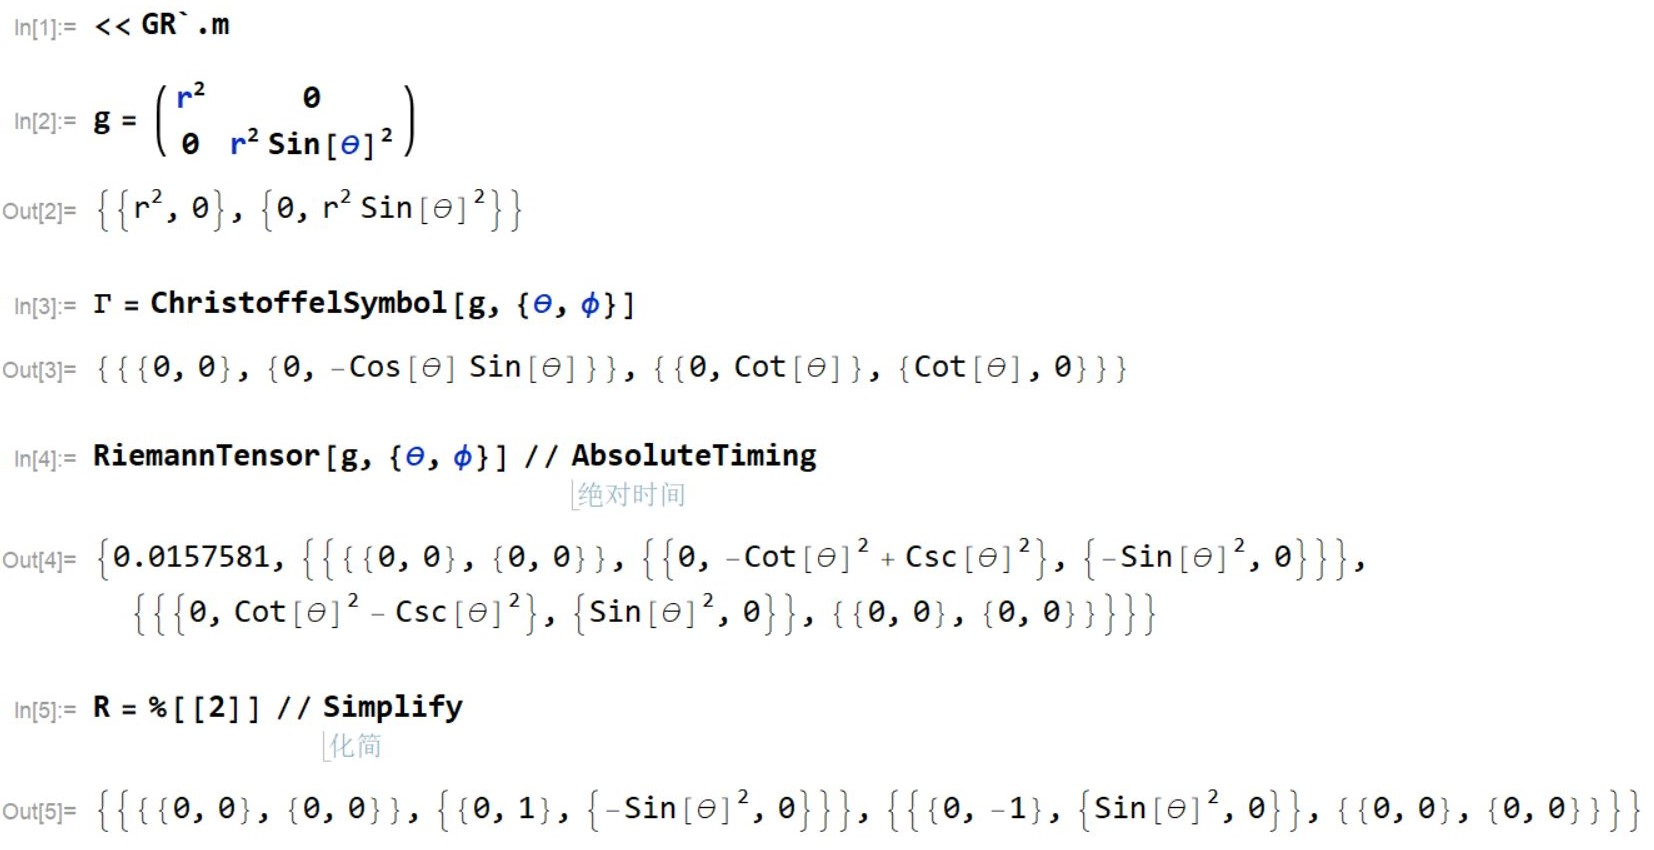
\includegraphics[width=0.8\textwidth]{pictures/1}
			\caption{将第13题扔给麦酱计算}\label{f3.1}
		\end{figure}
	\end{jie}
	
	\item \hypertarget{3.14}{}求度规$\dd{s}^2 = \Omega^2(t,x) \left(-\dd{t}^2 + \dd{x}^2\right) $的黎曼张量在$\{t,x\}$系的全部分量(在结果中以$\dot{\Omega} $和$ \Omega^\prime$ 分别代表函数 $\Omega$对$t$和$x$的偏导数)。
	
	\begin{jie}
		先求克氏符。
		\begin{align*}
		\ChristoffelSymbol{t}{t}{t} &= \christoffelSymbol{t}{t}{t}{t}\\
		&= \frac{\dot{\Omega}}{\Omega}\\
		\ChristoffelSymbol{t}{t}{x} &= \christoffelSymbol{t}{t}{x}{t}\\
		&= \frac{\Omega^\prime}{\Omega}\\
		\ChristoffelSymbol{t}{x}{x} &= \christoffelSymbol{t}{x}{x}{t}\\
		&= \frac{\dot{\Omega}}{\Omega}\\
		\ChristoffelSymbol{x}{t}{t} &= \christoffelSymbol{x}{t}{t}{x}\\
		&= \frac{\Omega^\prime}{\Omega}\\
		\ChristoffelSymbol{x}{t}{x} &= \christoffelSymbol{x}{t}{x}{x}\\ \displaybreak[1]
		&= \frac{\dot{\Omega}}{\Omega}\\
		\ChristoffelSymbol{x}{x}{x} &= \christoffelSymbol{x}{x}{x}{x}\\
		&= \frac{\Omega^\prime}{\Omega}
		\end{align*}
		则
		\begin{align*}
		\tensor{R}{_t_x_t^t}&= \riemannR{t}{x}{t}{t}{t} + \ChristoffelSymbol{x}{t}{t} \ChristoffelSymbol{t}{x}{x} - \ChristoffelSymbol{x}{t}{x} \ChristoffelSymbol{t}{t}{x}\\
		&= \frac{\Omega \dot{\Omega}^\prime - \dot{\Omega} \Omega^\prime}{\Omega^2} - \frac{\Omega \dot{\Omega}^\prime - \dot{\Omega} \Omega^\prime}{\Omega^2} + \frac{\dot{\Omega}\Omega^\prime}{\Omega^2} - \frac{\dot{\Omega}\Omega^\prime}{\Omega^2} + \frac{\dot{\Omega}\Omega^\prime}{\Omega^2} -\frac{\dot{\Omega}\Omega^\prime}{\Omega^2}\\
		&= 0\\
		\tensor{R}{_t_x_x^t}&=\riemannR{t}{x}{x}{t}{t}+ \ChristoffelSymbol{x}{x}{t} \ChristoffelSymbol{t}{x}{x}- \ChristoffelSymbol{x}{x}{x} \ChristoffelSymbol{t}{t}{x}\\
		&=\frac{\Omega\Omega^{\prime\prime}- {\Omega^{\prime}}^2}{\Omega^2}- \frac{\Omega\ddot{\Omega}- \dot{\Omega}^2}{\Omega^2}+ \frac{{\Omega^\prime}^2}{\Omega^2}- \frac{\dot{\Omega}^2}{\Omega^2}+ \frac{\dot{\Omega}^2}{\Omega^2}- \frac{{\Omega^\prime}^2}{\Omega^2}\\
		&=\frac{\Omega \left( \Omega^{\prime\prime}- \ddot{\Omega} \right)+ \dot{\Omega}^2 - {\Omega^\prime}^2 }{\Omega^2}\\
		\tensor{R}{_t_x_t^x}&= \riemannR{t}{x}{t}{x}{t}+ \ChristoffelSymbol{x}{t}{t} \ChristoffelSymbol{x}{x}{x}- \ChristoffelSymbol{x}{t}{x} \ChristoffelSymbol{x}{t}{x}\\
		&=\frac{\Omega\Omega^{\prime\prime}- {\Omega^\prime}^2}{\Omega^2}- \frac{\Omega\ddot{\Omega}- \dot{\Omega}^2}{\Omega^2} + \frac{\dot{\Omega}^2}{\Omega^2}- \frac{{\Omega^\prime}^2}{\Omega^2}+ \frac{{\Omega^\prime}^2}{\Omega^2}- \frac{\dot{\Omega}^2}{\Omega^2}\\
		&=\frac{\Omega \left( \Omega^{\prime\prime}- \ddot{\Omega} \right)+ \dot{\Omega}^2 - {\Omega^\prime}^2 }{\Omega^2}\\
		\tensor{R}{_t_x_x^x}&= \riemannR{t}{x}{x}{x}{t}+ \ChristoffelSymbol{x}{x}{t} \ChristoffelSymbol{x}{x}{x}- \ChristoffelSymbol{x}{x}{x} \ChristoffelSymbol{x}{t}{x}\\
		&=  \frac{\Omega \dot{\Omega}^\prime - \dot{\Omega} \Omega^\prime}{\Omega^2}-  \frac{\Omega \dot{\Omega}^\prime - \dot{\Omega} \Omega^\prime}{\Omega^2}+ \frac{\Omega^\prime\dot{\Omega}}{\Omega^2}- \frac{\Omega^\prime\dot{\Omega}}{\Omega^2}+ \frac{\Omega^\prime\dot{\Omega}}{\Omega^2}- \frac{\Omega^\prime\dot{\Omega}}{\Omega^2}\\
		&=0
		\end{align*}
		故所有非零分量为$\displaystyle \tensor{R}{_t_x_x^t}= -\tensor{R}{_x_t_x^t}=\tensor{R}{_t_x_t^x}= -\tensor{R}{_x_t_t^x}= \frac{\Omega \left( \Omega^{\prime\prime}- \ddot{\Omega} \right)+ \dot{\Omega}^2 - {\Omega^\prime}^2 }{\Omega^2} $。
		
		本题用上述Mathematica代码解决如图~\ref{f3.2}:
		\begin{figure}[htb]
			\centering
			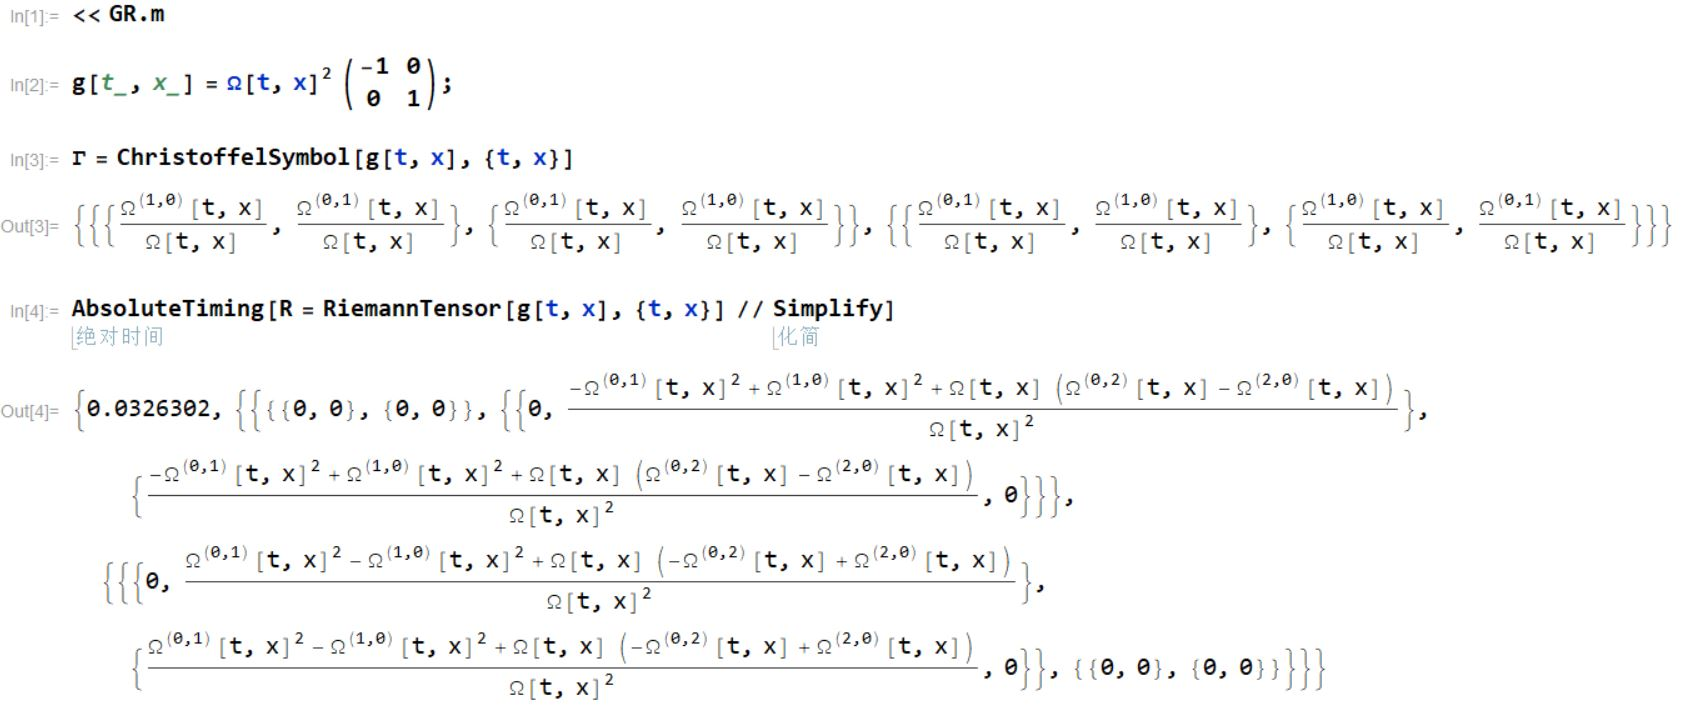
\includegraphics[width=0.8\textwidth]{pictures/2}
			\caption{将第14题扔给麦酱}\label{f3.2}
		\end{figure}
	\end{jie}
	
	\item \hypertarget{3.15}{}求度规$\dd{s}^2=z^{-1/2} \left(-\dd{t}^2+\dd{z}^2\right)+ z\left(\dd{x}^2+\dd{y}^2\right)$的黎曼张量在$\{t,x,y,z\}$系的全部分量。
	
	\begin{jie}
		先求克氏符分量。由度规分量的非对角元均为零,克氏符分量\[\ChristoffelSymbol{\sigma}{\mu}{\nu}=\christoffelSymbol{\sigma}{\mu}{\nu}{\sigma}\]。非零分量至少应该满足:$\sigma\mu\nu$至少有两个相等;$\sigma\mu\nu$中至少有一个为$z$(否则导数项全为零)。进一步地,若两个相等,则第三个必为$z$(否则导数项为零);若三个相等,则为$zzz$。即,非零分量满足三个指标中一个为$z$其余两个相同。
		\begin{align*}
		\ChristoffelSymbol{t}{t}{z}&= \christoffelSymbol{t}{t}{z}{t}\\
		&=-\frac{1}{4z}\\
		\ChristoffelSymbol{x}{x}{z}&= \christoffelSymbol{x}{x}{z}{x}\\
		&=\frac{1}{z}\\
		\ChristoffelSymbol{y}{y}{z}&= \christoffelSymbol{y}{y}{z}{y}\\
		&=\frac{1}{z}\\
		\ChristoffelSymbol{z}{t}{t}&= \christoffelSymbol{z}{t}{t}{z}\\
		&=-\frac{1}{4z}\\
		\ChristoffelSymbol{z}{x}{x}&= \christoffelSymbol{z}{x}{x}{z}\\
		&=-\frac{\sqrt{z}}{2}\\
		\ChristoffelSymbol{z}{y}{y}&= \christoffelSymbol{z}{y}{y}{z}\\
		&=-\frac{\sqrt{z}}{2}\\
		\ChristoffelSymbol{z}{z}{z}&= \christoffelSymbol{z}{z}{z}{z}\\
		&=-\frac{1}{4z}
		\end{align*}
		于是所有非零克氏符分量为$\displaystyle \ChristoffelSymbol{t}{t}{z}= \ChristoffelSymbol{t}{z}{t}= -\frac{1}{4z}$,$\displaystyle \ChristoffelSymbol{x}{x}{z}= \ChristoffelSymbol{x}{z}{x} = \ChristoffelSymbol{y}{y}{z}= \ChristoffelSymbol{y}{z}{y}= \frac{1}{z} $,$\displaystyle \ChristoffelSymbol{z}{t}{t}= -\frac{1}{4z}$, $\displaystyle \ChristoffelSymbol{z}{x}{x}= \ChristoffelSymbol{z}{y}{y}= -\frac{\sqrt{z}}{2} $, $\displaystyle \ChristoffelSymbol{z}{z}{z}= -\frac{1}{4z} $。
		
		由黎曼曲率张量分量表达式$\displaystyle \tensor{R}{_\mu_\nu_\sigma^\rho}= \ChristoffelSymbol{\rho}{\sigma}{{\mu,\nu}}- \ChristoffelSymbol{\rho}{\nu}{{\sigma,\mu}}+ \ChristoffelSymbol{\lambda}{\sigma}{\mu} \ChristoffelSymbol{\rho}{\nu}{\lambda}- \ChristoffelSymbol{\lambda}{\nu}{\sigma} \ChristoffelSymbol{\rho}{\mu}{\lambda} $,注意到上述克氏符非零项的规律,黎曼张量的非零分量至少应该满足 $\mu \neq \nu$并且:
		\begin{enumerate}
			\item $\rho$不为$z$时,导数项非零的条件是$\mu\nu$中有一个为$z$另一个和$\rho$相同且$\sigma=z$;下面分类讨论后两项。
			\begin{enumerate}
				\item $\mu\nu$中有一个为$z$时,设$\nu=z$,$\displaystyle \tensor{R}{_\mu_z_\sigma^\rho}= \ChristoffelSymbol{\rho}{\sigma}{{\mu,z}}- \cancel{\ChristoffelSymbol{\rho}{z}{{\sigma,\mu}}}+ \ChristoffelSymbol{\lambda}{\sigma}{\mu} \ChristoffelSymbol{\rho}{z}{\lambda}- \ChristoffelSymbol{\lambda}{z}{\sigma} \ChristoffelSymbol{\rho}{\mu}{\lambda} $,倒数第二项中$\rho z\lambda$的组合为满足克氏符非零项“一个为$z$其余两个相同”的特征,要求$\lambda=\rho$;最后一项中$\lambda z\sigma $的组合要求$\lambda=\sigma$,于是$\displaystyle \tensor{R}{_\mu_z_\sigma^\rho}= \ChristoffelSymbol{\rho}{\sigma}{{\mu,z}}+ \ChristoffelSymbol{\rho}{\sigma}{\mu} \ChristoffelSymbol{\rho}{z}{\rho}- \ChristoffelSymbol{\sigma}{z}{\sigma} \ChristoffelSymbol{\rho}{\mu}{\sigma} $,第一项非零要求$\mu=\rho$且$\sigma=z$,第二项非零要求$\mu=\rho $且$\sigma=z$;最后一项非零要求$\mu=\rho$且$\sigma=z$,于是非零项为$\displaystyle \tensor{R}{_\rho_z_z^\rho}= \ChristoffelSymbol{\rho}{z}{{\rho,z}}+ \ChristoffelSymbol{\rho}{z}{\rho} \ChristoffelSymbol{\rho}{z}{\rho}- \ChristoffelSymbol{z}{z}{z} \ChristoffelSymbol{\rho}{\rho}{z} $。
				\item $\mu\nu$均不为$z$时,求导项为零,$\displaystyle \tensor{R}{_\mu_\nu_\sigma^\rho}=  \ChristoffelSymbol{\lambda}{\sigma}{\mu} \ChristoffelSymbol{\rho}{\nu}{\lambda}- \ChristoffelSymbol{\lambda}{\nu}{\sigma} \ChristoffelSymbol{\rho}{\mu}{\lambda} $,第一项中$\rho\nu\lambda$的组合要求$\lambda=z $且$\nu=\rho $,第二项中$\rho\mu\lambda$的组合要求$\lambda=z$且$\mu=\rho$,于是$\displaystyle \tensor{R}{_\mu_\nu_\sigma^\rho}=  \ChristoffelSymbol{z}{\sigma}{\mu} \ChristoffelSymbol{\rho}{\nu}{z}- \ChristoffelSymbol{z}{\nu}{\sigma} \ChristoffelSymbol{\rho}{\mu}{z} $,$\mu\nu$中至少一个与$\rho$相同。不妨设$\mu=\rho$,则$\displaystyle \tensor{R}{_\rho_\nu_\sigma^\rho}=- \ChristoffelSymbol{z}{\nu}{\sigma} \ChristoffelSymbol{\rho}{\rho}{z} $,非零项为$\displaystyle \tensor{R}{_\rho_\nu_\nu^\rho}=- \ChristoffelSymbol{z}{\nu}{\nu} \ChristoffelSymbol{\rho}{\rho}{z} $。
			\end{enumerate}
			\item $\rho$为$z$时,则后两项中$\lambda$应分别取$\nu$和$\mu$,即$\displaystyle \tensor{R}{_\mu_\nu_\sigma^z}= \ChristoffelSymbol{z}{\sigma}{{\mu,\nu}}- \ChristoffelSymbol{z}{\nu}{{\sigma,\mu}}+ \ChristoffelSymbol{\nu}{\sigma}{\mu} \ChristoffelSymbol{z}{\nu}{\nu}- \ChristoffelSymbol{\mu}{\nu}{\sigma} \ChristoffelSymbol{z}{\mu}{\mu} $,若$\mu\nu$均不为$z$,则导数项为零,而后两项中$\ChristoffelSymbol{\nu}{\sigma}{\mu}$和$ \ChristoffelSymbol{\mu}{\nu}{\sigma} $无论$\sigma$如何取都不能满足克氏符非零项“一个为$z$其余两个相同”的特征,故$\mu \nu$中有一个为$z$,考虑到指标$\mu \nu$反称只需计算偶排列,于是我们有$\nu=z$,非零项为$\displaystyle \tensor{R}{_\mu_z_\sigma^z}= \ChristoffelSymbol{z}{\sigma}{{\mu,z}}+ \ChristoffelSymbol{z}{\sigma}{\mu} \ChristoffelSymbol{z}{z}{z}- \ChristoffelSymbol{\mu}{z}{\sigma} \ChristoffelSymbol{z}{\mu}{\mu} $,又看出必须有$\mu= \sigma$,于是非零项为$\displaystyle \tensor{R}{_\mu_z_\mu^z}= \ChristoffelSymbol{z}{\mu}{{\mu,z}}+ \ChristoffelSymbol{z}{\mu}{\mu} \ChristoffelSymbol{z}{z}{z}- \ChristoffelSymbol{\mu}{z}{\mu} \ChristoffelSymbol{z}{\mu}{\mu} $。
		\end{enumerate} 
	综上,可能非零项为
	\begin{align*}
	\tensor{R}{_\rho_z_z^\rho}&= \ChristoffelSymbol{\rho}{z}{{\rho,z}}+ \ChristoffelSymbol{\rho}{z}{\rho} \ChristoffelSymbol{\rho}{z}{\rho}- \ChristoffelSymbol{z}{z}{z} \ChristoffelSymbol{\rho}{\rho}{z}, & \rho&=t,x,y\\
	\tensor{R}{_\rho_\nu_\nu^\rho}&=- \ChristoffelSymbol{z}{\nu}{\nu} \ChristoffelSymbol{\rho}{\rho}{z}, & \rho,\nu&=t,x,y \\
	\tensor{R}{_\mu_z_\mu^z}&= \ChristoffelSymbol{z}{\mu}{{\mu,z}}+ \ChristoffelSymbol{z}{\mu}{\mu} \ChristoffelSymbol{z}{z}{z}- \ChristoffelSymbol{\mu}{z}{\mu} \ChristoffelSymbol{z}{\mu}{\mu}, & \mu&=t,x,y.
	\end{align*}
	又注意到$x$与$y$的对称性,只需计算$x$而不用计算$y$、只需计算$xyyx$不用计算$yxxy$。下面按以上规则计算可能的非零分量。
	\begin{align*}
	\tensor{R}{_t_x_x^t}&=- \ChristoffelSymbol{z}{x}{x} \ChristoffelSymbol{t}{t}{z}\\ \displaybreak[1]
	&=-\frac{1}{8\sqrt{z}}\\
	\tensor{R}{_t_z_z^t}&= \ChristoffelSymbol{t}{z}{{t,z}}+ \ChristoffelSymbol{t}{z}{t} \ChristoffelSymbol{t}{z}{t}- \ChristoffelSymbol{z}{z}{z} \ChristoffelSymbol{t}{t}{z}\\
	&= \frac{1}{4z^2} +\frac{1}{16z^2}-\frac{1}{16z^2} \\ \displaybreak[1]
	&= \frac{1}{4z^2}\\
	\tensor{R}{_x_y_y^x}&=- \ChristoffelSymbol{z}{y}{y} \ChristoffelSymbol{x}{x}{z}\\ \displaybreak[1]
	&=\frac{1}{4\sqrt{z}}\\
	\tensor{R}{_x_z_z^x}&= \ChristoffelSymbol{x}{z}{{x,z}}+ \ChristoffelSymbol{x}{z}{x} \ChristoffelSymbol{x}{z}{x}- \ChristoffelSymbol{z}{z}{z} \ChristoffelSymbol{x}{x}{z}\\
	&=-\frac{1}{2z^2}+ \frac{1}{4z^2}+ \frac{1}{8z^2}\\ \displaybreak[1]
	&=-\frac{1}{8z^2}\\
	\tensor{R}{_t_z_t^z}&= \ChristoffelSymbol{z}{t}{{t,z}}+ \ChristoffelSymbol{z}{t}{t} \ChristoffelSymbol{z}{z}{z}- \ChristoffelSymbol{t}{z}{t} \ChristoffelSymbol{z}{t}{t}\\
	&=\frac{1}{4z^2}+\frac{1}{16z^2}- \frac{1}{16z^2}\\ \displaybreak[1]
	&=\frac{1}{4z^2}\\
	\tensor{R}{_x_z_x^z}&= \ChristoffelSymbol{z}{x}{{x,z}}+ \ChristoffelSymbol{z}{x}{x} \ChristoffelSymbol{z}{z}{z}- \ChristoffelSymbol{x}{z}{x} \ChristoffelSymbol{z}{x}{x}\\
	&=-\frac{1}{4\sqrt{z}}+\frac{1}{8\sqrt{z}}+\frac{1}{4\sqrt{z}}\\
	&=\frac{1}{8\sqrt{z}}
	\end{align*}
	于是所有非零分量为
	\begin{align*}
	\tensor{R}{_t_x_x^t}&=-\tensor{R}{_x_t_x^t}=\tensor{R}{_t_y_y^t}= - \tensor{R}{_y_t_y^t}=-\frac{1}{8\sqrt{z}}\\
	\tensor{R}{_t_z_z^t}&=-\tensor{R}{_z_t_z^t}=\frac{1}{4z^2}\\
	\tensor{R}{_x_y_y^x}&=\tensor{R}{_y_x_x^y}=\frac{1}{4\sqrt{z}}\\
	\tensor{R}{_x_z_z^x}&=-\tensor{R}{_z_x_z^x}= \tensor{R}{_y_z_z^y}=-\tensor{R}{_z_y_z^y}=-\frac{1}{8z^2}\\
	\tensor{R}{_t_z_t^z}&=-\tensor{R}{_z_t_t^z}=\frac{1}{4z^2}\\
	\tensor{R}{_x_z_x^z}&=-\tensor{R}{_z_x_x^z}=\frac{1}{8\sqrt{z}}
	\end{align*}
	PS:我第一遍手算的算了几个小时(论经常抄错指标的悲惨……)所以还是分析一番,分类讨论分量非零条件顺便化简的好……当然最省事的还是交给麦酱,秒出结果……
	\end{jie}
	
	\item \hypertarget{3.16}{}设$\alpha(z)$,$\beta(z)$,$\gamma(z)$为任意函数,$h=t+ \alpha(z)x+\beta(z)y+\gamma(z) $,求度规\[ \dd{s}^2= -\dd{t}^2 + \dd{x}^2 +\dd{y}^2 +h^2\dd{z}^2 \] 的黎曼张量在$\{t,x,y,z\}$系的全部分量。
	
	\begin{jie}
		首先求克氏符分量,由于度规分量矩阵的非对角元全为零,\[\displaystyle \ChristoffelSymbol{\sigma}{\mu}{\nu}=\christoffelSymbol{\sigma}{\mu}{\nu}{\sigma}\],导数项非零要求$\sigma\mu\nu$中有两个取$z$。
		\begin{align*}
		\ChristoffelSymbol{t}{z}{z}&=\christoffelSymbol{t}{z}{z}{t}\\ \displaybreak[1]
		&= h\\
		\ChristoffelSymbol{x}{z}{z}&=\christoffelSymbol{x}{z}{z}{x}\\ \displaybreak[1]
		&=-h\alpha\\
		\ChristoffelSymbol{y}{z}{z}&=\christoffelSymbol{y}{z}{z}{y}\\ \displaybreak[1]
		&=-h\beta\\
		\ChristoffelSymbol{z}{z}{t}&=\christoffelSymbol{z}{z}{t}{z}\\ \displaybreak[1]
		&=\frac{1}{h}\\
		\ChristoffelSymbol{z}{z}{x}&=\christoffelSymbol{z}{z}{x}{z}\\ \displaybreak[1]
		&=\frac{\alpha}{h}\\
		\ChristoffelSymbol{z}{z}{y}&= \christoffelSymbol{z}{z}{y}{z}\\ \displaybreak[1]
		&=\frac{\beta}{h}\\
		\ChristoffelSymbol{z}{z}{z}&=\christoffelSymbol{z}{z}{z}{z}\\
		&=\frac{x\alpha^\prime+y\beta^\prime+\gamma^\prime}{h}
		\end{align*}
		黎曼张量分量表达式为$\displaystyle \tensor{R}{_\mu_\nu_\sigma^\rho}= \ChristoffelSymbol{\rho}{\sigma}{{\mu,\nu}}- \ChristoffelSymbol{\rho}{\nu}{{\sigma,\mu}}+ \ChristoffelSymbol{\lambda}{\sigma}{\mu} \ChristoffelSymbol{\rho}{\nu}{\lambda}- \ChristoffelSymbol{\lambda}{\nu}{\sigma} \ChristoffelSymbol{\rho}{\mu}{\lambda} $,下面讨论分量非零条件。
		\begin{enumerate}
			\item $\rho$不取$z$。后两项求和中$\lambda=z$,且$\mu\nu$必有一取$z$。由于前两个指标反称,设$\nu$取$z$,则$\displaystyle \tensor{R}{_\mu_z_\sigma^\rho}= \cancel{\ChristoffelSymbol{\rho}{\sigma}{{\mu,z}}}- \ChristoffelSymbol{\rho}{z}{{\sigma,\mu}}+ \ChristoffelSymbol{z}{\sigma}{\mu} \ChristoffelSymbol{\rho}{z}{z}- \ChristoffelSymbol{z}{z}{\sigma} \cancel{\ChristoffelSymbol{\rho}{\mu}{z}} $,又可看出$\sigma=z$,于是非零分量为$\displaystyle \tensor{R}{_\mu_z_z^\rho}=- \ChristoffelSymbol{\rho}{z}{{z,\mu}}+ \ChristoffelSymbol{z}{z}{\mu} \ChristoffelSymbol{\rho}{z}{z} $。
			\item $\rho$取$z$。
			\begin{enumerate}
				\item $\nu$取$z$。则$\displaystyle \tensor{R}{_\mu_z_\sigma^z}= \ChristoffelSymbol{z}{\sigma}{{\mu,z}}- \ChristoffelSymbol{z}{z}{{\sigma,\mu}}+ \ChristoffelSymbol{\lambda}{\sigma}{\mu} \ChristoffelSymbol{z}{z}{\lambda}- \ChristoffelSymbol{\lambda}{z}{\sigma} \ChristoffelSymbol{z}{\mu}{\lambda} $,倒数第二项中$\lambda\sigma\mu $的组合要求$\lambda=z$,最后一项中$z\mu\lambda$的组合要求$\lambda=z$。
				\begin{enumerate}
					\item $\sigma=z$,则$\displaystyle \tensor{R}{_\mu_z_z^z}= \ChristoffelSymbol{z}{z}{{\mu,z}}- \ChristoffelSymbol{z}{z}{{z,\mu}}+\cancel{\ChristoffelSymbol{z}{z}{\mu} \ChristoffelSymbol{z}{z}{z}- \ChristoffelSymbol{z}{z}{z} \ChristoffelSymbol{z}{\mu}{z}}  $;
					\item $\sigma\neq z$,则$\displaystyle \tensor{R}{_\mu_z_\sigma^z}= \cancel{\ChristoffelSymbol{z}{\sigma}{{\mu,z}}}- \ChristoffelSymbol{z}{z}{{\sigma,\mu}}+ \cancel{\ChristoffelSymbol{z}{\sigma}{\mu}} \ChristoffelSymbol{z}{z}{z}- \ChristoffelSymbol{z}{z}{\sigma} \ChristoffelSymbol{z}{\mu}{z} $。
				\end{enumerate}
			\item $\mu\nu$均不取$z$。则$\displaystyle \tensor{R}{_\mu_\nu_\sigma^z}= \ChristoffelSymbol{z}{\sigma}{{\mu,\nu}}- \ChristoffelSymbol{z}{\nu}{{\sigma,\mu}}+ \ChristoffelSymbol{\lambda}{\sigma}{\mu} \ChristoffelSymbol{z}{\nu}{\lambda}- \ChristoffelSymbol{\lambda}{\nu}{\sigma} \ChristoffelSymbol{z}{\mu}{\lambda} $,后两项中$\lambda$均取$z$,且$\sigma=z$。则$\displaystyle \tensor{R}{_\mu_\nu_z^z}= \ChristoffelSymbol{z}{z}{{\mu,\nu}}- \ChristoffelSymbol{z}{\nu}{{z,\mu}}+ \cancel{\ChristoffelSymbol{z}{z}{\mu} \ChristoffelSymbol{z}{\nu}{z}- \ChristoffelSymbol{z}{\nu}{z} \ChristoffelSymbol{z}{\mu}{z}} $。
			\end{enumerate}
		\end{enumerate}
	综上,仅考虑哪些克氏符非零,可以将可能的非零分量确定到如下四种情况:
	\begin{align*}
	\tensor{R}{_\mu_z_z^\rho}&=- \ChristoffelSymbol{\rho}{z}{{z,\mu}}+ \ChristoffelSymbol{z}{z}{\mu} \ChristoffelSymbol{\rho}{z}{z}, & \mu,\rho&=t,x,y \\
	\tensor{R}{_\mu_z_z^z}&= \ChristoffelSymbol{z}{z}{{\mu,z}}- \ChristoffelSymbol{z}{z}{{z,\mu}}, & \mu&=t,x,y \\
	\tensor{R}{_\mu_z_\sigma^z}&=- \ChristoffelSymbol{z}{z}{{\sigma,\mu}}- \ChristoffelSymbol{z}{z}{\sigma} \ChristoffelSymbol{z}{\mu}{z}, & \mu,\sigma&=t,x,y \\
	\tensor{R}{_\mu_\nu_z^z}&= \ChristoffelSymbol{z}{z}{{\mu,\nu}}- \ChristoffelSymbol{z}{\nu}{{z,\mu}}, & \mu,\nu&=t,x,y
	\end{align*}
	但是进一步考虑那些非零的克氏符分量的具体形式,由于\[\ChristoffelSymbol{z}{z}{\mu}= \frac{\pdv{h}{x^\mu}}{h},\]于是\[ \ChristoffelSymbol{z}{z}{{\mu,\nu}}=- \frac{\pdv{h}{x^\mu}\pdv{h}{x^\nu}}{h^2}= \ChristoffelSymbol{z}{z}{{\nu,\mu}}= \ChristoffelSymbol{z}{z}{\mu} \ChristoffelSymbol{z}{z}{\nu},\]故第二三四种情况均为零,还剩下\[
	\tensor{R}{_\mu_z_z^\rho}=- \ChristoffelSymbol{\rho}{z}{{z,\mu}}+ \ChristoffelSymbol{z}{z}{\mu} \ChristoffelSymbol{\rho}{z}{z}\qc\quad \rho=t,x,y \]
	而\[ \ChristoffelSymbol{\rho}{z}{z}=-\tensor{g}{^\rho^\rho} h \pdv{h}{x^\rho} \]可以观察发现
	\begin{align*}
	\ChristoffelSymbol{\rho}{z}{{z,\mu}}&=-\tensor{g}{^\rho^\rho}\pdv{h}{x^\rho} \pdv{h}{x^\mu}\\
	&=\left(-\tensor{g}{^\rho^\rho} h \pdv{h}{x^\mu}\right) \left(\frac{\pdv{h}{x^\mu}}{h}\right)\\
	&=\ChristoffelSymbol{z}{z}{\mu} \ChristoffelSymbol{\rho}{z}{z}
	\end{align*}
	于是本题的黎曼张量的所有分量全为零。扔给麦酱验证如图~\ref{f3.3}
	\begin{figure}[htb]
		\centering
		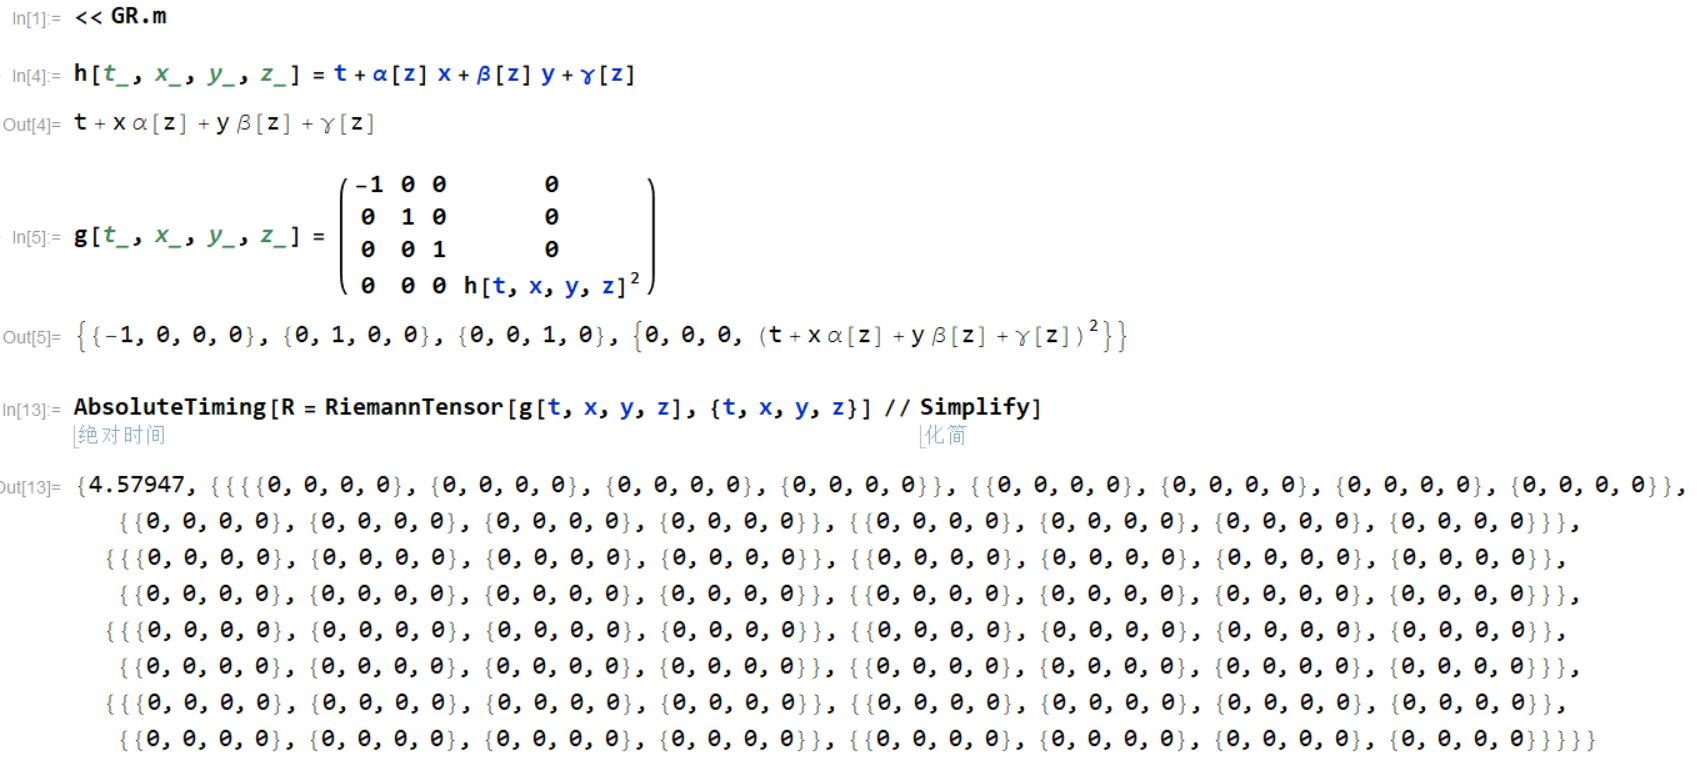
\includegraphics[width=0.8\textwidth]{pictures/3}
		\caption{Mathematica验证第16题}\label{f3.3}
	\end{figure}
	\end{jie}
	
	\item 试证2维广义黎曼空间的爱因斯坦张量为零。提示:2维广义黎曼空间的黎曼张量只有一个独立分量。
	
	\begin{zm}
		记$r\equiv\tensor{R}{_1_2_1_2} $,则
		\begin{align*}
		\tensor{R}{_2_1_1_2}&=-r\\
		\tensor{R}{_1_2_2_1}&=-r\\
		\tensor{R}{_2_1_2_1}&=r
		\end{align*}
		于是里奇张量$\tensor{R}{_a_c}:=\tensor{g}{^b^d} \tensor{R}{_a_b_c_d}$的分量为
		\begin{align*}
		\tensor{R}{_1_1}&=\tensor{g}{^2^2} \tensor{R}{_1_2^1_2}\\ \displaybreak[1]
		&=r\tensor{g}{^2^2}\\
		\tensor{R}{_1_2}&=\tensor{g}{^2^1} \tensor{R}{_1_2_2_1}\\ \displaybreak[1]
		&=-r\tensor{g}{^2^1}\\
		\tensor{R}{_2_2}&=\tensor{g}{^1^1} \tensor{R}{_2_1_2_1}\\
		&=r\tensor{g}{^1^1},
		\end{align*}
		标量曲率
		\begin{align*}
		R&=\tensor{g}{^a^c} \tensor{R}{_a_c}\\
		&=2r\tensor{g}{^1^1} \tensor{g}{^2^2} -2r \tensor{g}{^1^2} \tensor{g}{^2^1} \\
		&=2rg.
		\end{align*}
		其中$g=\det [g]$为度规分量矩阵的行列式。注意到,里奇张量分量排成的矩阵为
		\begin{align*}
		\left[R\right]&=\left( 
		\begin{array}{cc}
		r\tensor{g}{^2^2}&-r\tensor{g}{^2^1}\\
		-r\tensor{g}{^1^2}&r\tensor{g}{^1^1}
		\end{array}
		\right)\\
		&=r\left([g]^{-1}\right)^*\\
		&=rg[g],
		\end{align*}
		其中$A^*$代表$A$的伴随矩阵。于是爱因斯坦张量$ \displaystyle \tensor{G}{_a_b}=\tensor{R}{_a_b}-\frac{1}{2} R \tensor{g}{_a_b}$的分量矩阵为
		\begin{align*}
		[G]&=[R]-\frac{1}{2} R [g]\\
		&=rg[g]-rg[g]\\
		&=0.
		\end{align*}
	\end{zm}
	
	
	
\end{xiti}